\documentclass[a4paper]{article}
\usepackage[latin1]{inputenc}
\usepackage{graphicx}
\usepackage{array}
\usepackage{amsmath}
\newcommand{\transp}{\top}

\usepackage{caption}
\usepackage{subcaption}

\setlength{\parskip}{2ex}

\begin{document}


\title{Independent Study Report - CB + DMPs}
\author{Francisco M. Garcia}
%\date{}

\maketitle


\section{Introduction}

\indent \indent In this independent study, I focused my attention to two related approaches to motor control: Control Basis (CB) and Dynamic Movement Primitives (DMPs). CB provides a way of generating complex movement from a sequential composition of simple primitives, while DMPs is a parametric model that allows the reproduction and generalization of demonstrations. In this work, I studied the feasibility of a hybrid approach in which CB provides an unsupervised method for generating movements and DMPs generalize and improves the demonstration.

\section{Control Basis}

In this se

\section{Dynamic Movement Primitives}

\indent \indent Dynamic Movement Primitives (DMPs) provide a general approach for learning robotic motor skill from demonstration. Given a sample trajectory with start state $x_0$ and goal state $g$, a DMP generates a trajectory by integrating the following equations:

$$
\tau \dot{v} = K(g - x) - Dv - K(g - x_0) s + Kf(s)
$$
$$
\tau \dot{x} = v
$$

In these equations, $\tau$ refers to a time scaling term, $K$ and $D$ refer on system specific constant that work as in a PD controller and $f(s)$ corresponds to a non-linear function composed of several Gaussian basis functions:

$$
f(s) = \frac{\sum_i w_i \psi_i(s) s }{\sum_i \psi_i(s)}
$$

where $\psi_i(s) = \exp(-h_i(s-c_i)^2)$ are the basis functions with center $c_i$ and width $h_i$. $w_i$ are the parameters to be found to minimize the objective function J. \\
\indent The variable $s$ is a phase variable which encompases the duration of the trajectory and monotonically decreases from 1 to 0. This variable obtained by the canonical system:
$$
\tau \dot{s} = -\alpha s
$$
 
When observing a demonstration, a movement $x(t)$ is recorded and from that its derivative $v(t)$ and $\dot{v}$ are obtained. Using this, we can compute the target function:
$$
f_{target}(s) = \frac{\tau \dot{v} + Dv}{K} - (g - x) + (g - x_0) s
$$ 

and solve the objective function $J = \sum_s (f_{target}(s) - f(s))^2$ via gradient descent or least-squares. \\
\indent Once trained, a new trajectory can be generated by setting $s$ to 1, updating the positions and velocities and intergrating the canonical system to obtained the new $s$.

Figure \ref{fig:test} shows the plot of DMPs for a 2-link robotic arm simulator. The x-axis is time measured in seconds, while the y-axis measures the angular position in radians. The line in red is the trajectory of the demonstration, while the line in blue is the approximation generated from the DMP. In this case, the DMPs are set to the same initial and goal positions, so as to recreate the same movement.  
 
 
\begin{figure}
\centering
\begin{subfigure}{.5\textwidth}
  \centering
  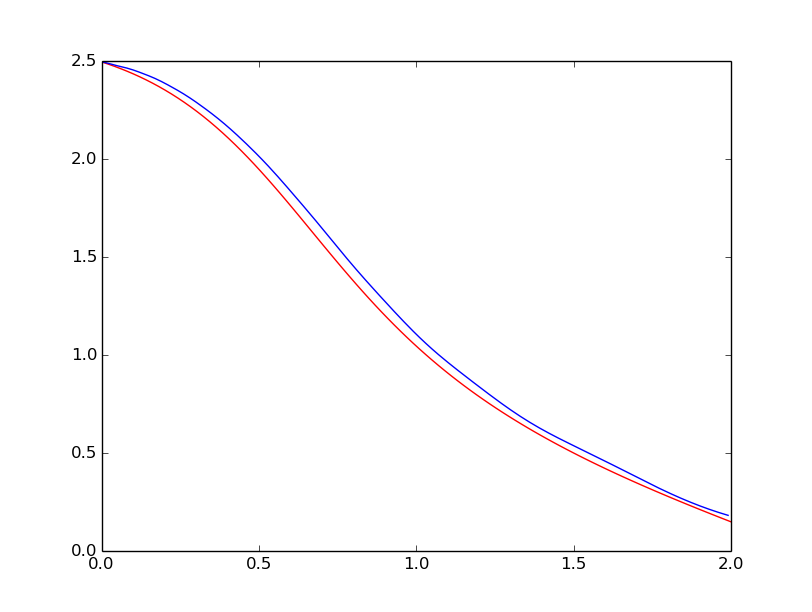
\includegraphics[width=.8\linewidth]{figure_1.png}
  \caption{DMP for joint 1}
  \label{fig:sub1}
\end{subfigure}%
\begin{subfigure}{.5\textwidth}
  \centering
  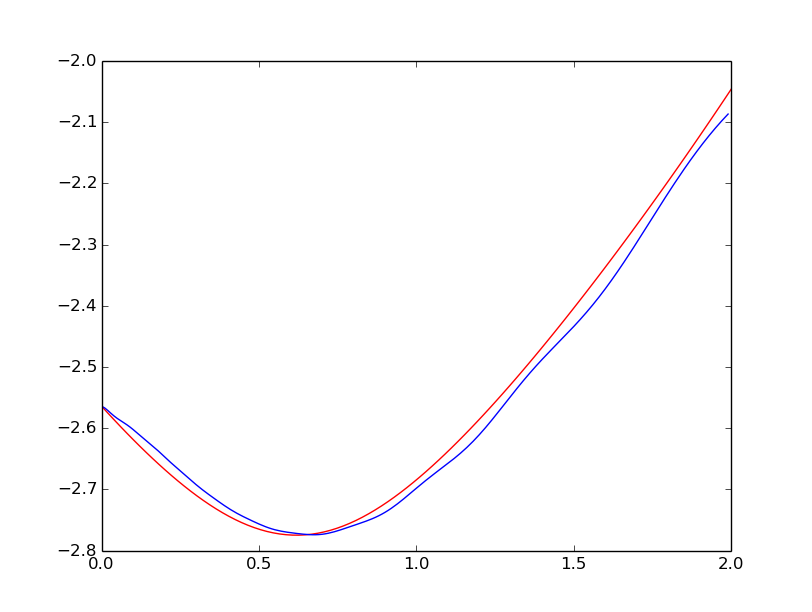
\includegraphics[width=.8\linewidth]{figure_2.png}
  \caption{DMP for joint 2}
  \label{fig:sub2}
\end{subfigure}
\caption{Plot of demonstrations and their corresponding DMP}
\label{fig:test}
\end{figure}

\section{Combining CB and DMPs}
 
 
\end{document}